%!TEX root = ./main.tex

\section{Experiments}

\paragraph{Setting.}
To evaluate the empirical performance of our proposed algorithm, we conducted experiments on routing problems
that are motivated by congestion management.
In this problem we are given a directed graph $G(A,V)$ and a set of requests $R = \{(s_{i}, t_{i}) : s_{i}, t_{i} \in V\}$ that represents demands to connect $s_{i}$ to $t_{i}$. We assume that for each request there exists a directed path between $s_{i}$ to $t_{i}$.
Each arc $(u, v) \in A$ is associated with a cost function $f_{(u,v)}: \mathbb{R}^{+} \rightarrow \mathbb{R}^{+}$ that depends on the number of requests using the arc.
Requests arrive online and the goal is to design a routing that minimizes the total cost.


\paragraph{Input.}
There are three type of inputs in our experiments. The first one includes randomly generated graphs following the Erd\H{o}s-Rényi model $G(n, p)$, where $n$ is the number of vertices and $p$ is the probability that an arc gets created. The source and target vertices of the requests are also generated uniformly at random. The second category creates a cycle with $n$ vertices and creates an arc between each neighboring vertex in both direction, ensuring that each vertex is connected. Afterwards, we randomly generate edges between non-adjacent vertices, as well as the requests.
The third input type collects specific examples designed to trap algorithms which rely on the multiplicative weight update (MWU) method. These instances do not include randomness, they were designed by hand.


\paragraph{Predictions.}
The predictions come from rounding the optimal offline fractional solution. If a request is served by several paths in the fractional solution, the oracle picks one of the paths uniformly at random using the amounts passing through each of them as weights. Otherwise, the oracle uses the unique best path of the optimal solution. Due to the randomized rounding, on most instances the oracles propose a worse solution than the multiplicative weight update (MWU) solution. To improve the quality of the oracles, we create several unique oracles and then take the ones with the best, the worst and the middle performance during our analysis.


\paragraph{Implementation.}
The routing problem's covering formulation enumerates all possible cuts in the graph. Upon each arriving request $r = (s,t)$, a new set of constraints are released $\sum_{e \in \delta(S)} x_{e}^{r} \ge 1$, where $\delta(S)$ is the cut on $S \subset V$ such that $s \in S$ and $t \notin S$. This formulation generates an exponential number of constraints with respect to the size of the graph. However, these constraints can be simplified in the implementation of Algorithm~\ref{algo:covering}, since the algorithm is not constrained by standard linear program solving techniques. Algorithm~\ref{algo:covering} increases the amount of traffic on each arc following the step described on line \ref{algo-covering:x}. The request is satisfied when there exists a path among the arcs in the set $A^{*}$ (arcs with value $1$). Therefore, we can replace the constraint satisfaction with a simple path finding in the implementation. If there are several possible paths with the arcs in $A^{*}$, our algorithm chooses the minimum cost path, so the implementation includes a rounding step, providing an integral solution.


\paragraph{Instances.} Randomly generated instances yield similar results. On large instances with many vertices, arcs, and request, the multiplicative weight update (MWU) solution and the oracles are far from the optimal offline fractional solution. However, on small instances, the MWU works well, and it is more likely to obtain good oracles. Instance $1$ represents a large randomly generated instance, while Instance $2$ a small one. The second category of inputs guarantee that the graph is connected and Instance $3$ represents on of these inputs. Finally, we show an example, where the MWU makes really sub-optimal decisions on Instance $4$. These instances are complementary and allow us to examine how our algorithm behaves when the oracles' predictions are worse or better than the MWU.

\textit{Instance $1$} has $20$ vertices, $184$ arcs, and $20$ requests. Each arc has a cost function of the form $f(x) = a x^b$, where $1.0 \le a \le 10.0$ and $1.0 \le b \le 4.0$. We generated $20$ oracles from the optimal offline fractional solution and kept $3$ of these oracles: the best, the worst and the middle one on the scale of their obtained objective values. The result of this execution is visible on \cref{fig:random}.

\textit{Instance $2$} has $10$ vertices, $32$ arcs, and $5$ requests. Each arc has a cost function of the form $f(x) = a x^b$, where $1.0 \le a \le 10.0$ and $1.0 \le b \le 4.0$. We generated $10$ oracles from the optimal offline fractional solution and kept $3$ of these oracles: the best, the worst and the middle one on the scale of their obtained objective values. The result of this execution is visible on \cref{fig:small-random}.

\textit{Instance $4$} has $50$ vertices, $120$ arcs, and $20$ requests. Each arc has a cost function of the form $f(x) = a x^b$, where $1.0 \le a \le 5.0$ and $1.0 \le b \le 5.0$. We generated $20$ oracles from the optimal offline fractional solution and kept $3$ of these oracles: the best, the worst and the middle one on the scale of their obtained objective values. The result of this execution is visible on \cref{fig:connected}.

\textit{Instance $4$} has $8$ vertices, $16$ arcs, and $7$ requests. This instance is specifically designed to trap the MWU. The structure of Instance $4$ is visible on \cref{fig:cex}, along with its MWU and optimal solutions.


\paragraph{Figures.} Each of the presented performance analysis figures have $eta$ on the x-axis, which represents the algorithm's trust in the predictions ($\eta = 0$ means the highest trust). The y-axis show the competitive ratio, which we have computed as the ratio between the optimal offline fractional solution and the algorithm's solution. The y-axis do not contain the complete range of values from $0$ to $1$ to make the figures smaller.

\paragraph{Observation.} Our algorithm updates the problem's variables following a combination of the multiplicative weight update (MWU) method and the oracle's predictions. When the predictions have an impact on the update of the variables ($eta$ tends towards $0$), and the quality of the predictions are good, our algorithm has a better performance.

Based on the experiments that we have conducted, we can remark that even if the oracle's performance are much worse than the MWU's performance, our algorithm's performance degrades gradually (see \cref{fig:small-random}). Additionally, if the oracle tries to give adversarial inputs (for example oracle $3$ on \cref{fig:random}), the algorithm may ignore the suggestions completely (the increasing rate coming from the oracle does not compensate the increasing rate difference due to the costs of the arcs).

Instance $4$ (which serves as a hand-crafted counter-example for the MWU) shows that the MWU method avoids taking a path which cost slightly more than the minimum cost path. As a result, our algorithm can only improve its performance, when its trust is high in the prediction. In this specific example, there is only one possible oracle, since the optimal offline fractional solution is already integral. Therefore, on \cref{fig:cex-perf} the columns are identical.

On some examples, both the multiplicative weight update and the oracle performs poorly (third column on \cref{fig:connected}), but their combination produces a good result. We can also remark that even if the oracle suggests a much better solution than the one the multiplicative weight update can obtain alone, our algorithm does not always follow blindly the oracle (first column of \cref{fig:connected}). Additionally, due to the way we increase the value of the variables (see line \ref{algo-covering:x} of the algorithm), in the setting of the routing problem, longer paths are penalized, even if they have a smaller cost. These observations suggest that the way we have integrated the predictions with the multiplicative weight update might be too simple to capture the necessary detail for specific problems. However, it provides a general framework with a worst-case guarantee that other people can build upon when they are studying specific problems.

{
    \begin{minipage}{0.3\textwidth}
        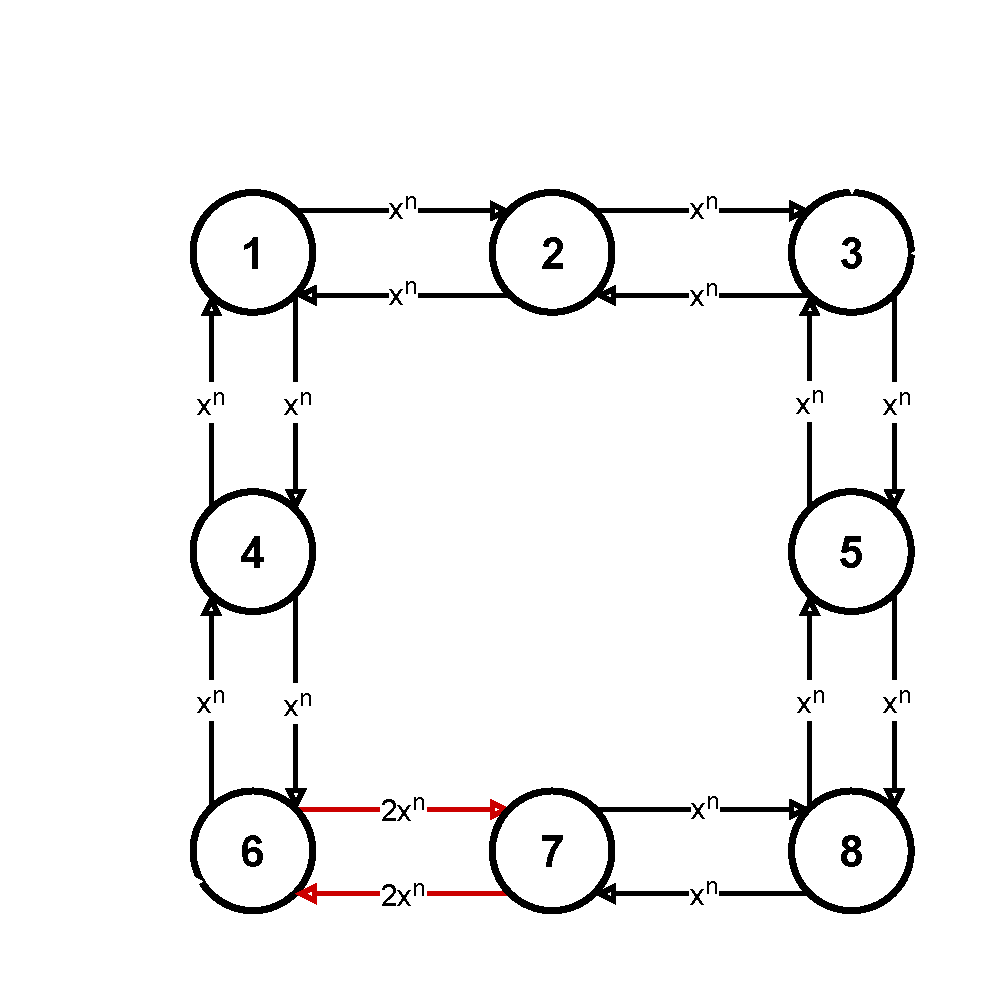
\includegraphics[width=\linewidth]{Img/cex_init.pdf}
    \end{minipage}
    \begin{minipage}{0.3\textwidth}
        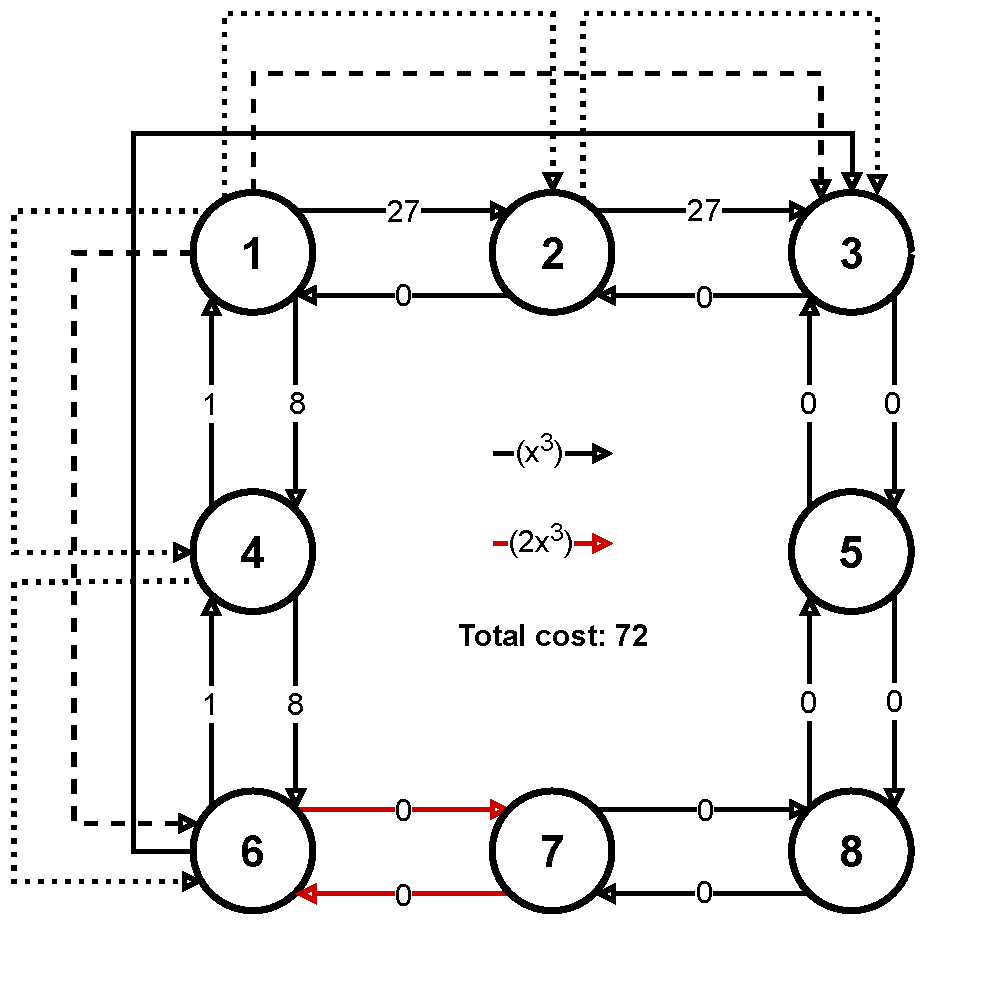
\includegraphics[width=\linewidth]{Img/cex_greedy.pdf}
    \end{minipage}
    \begin{minipage}{0.3\textwidth}
        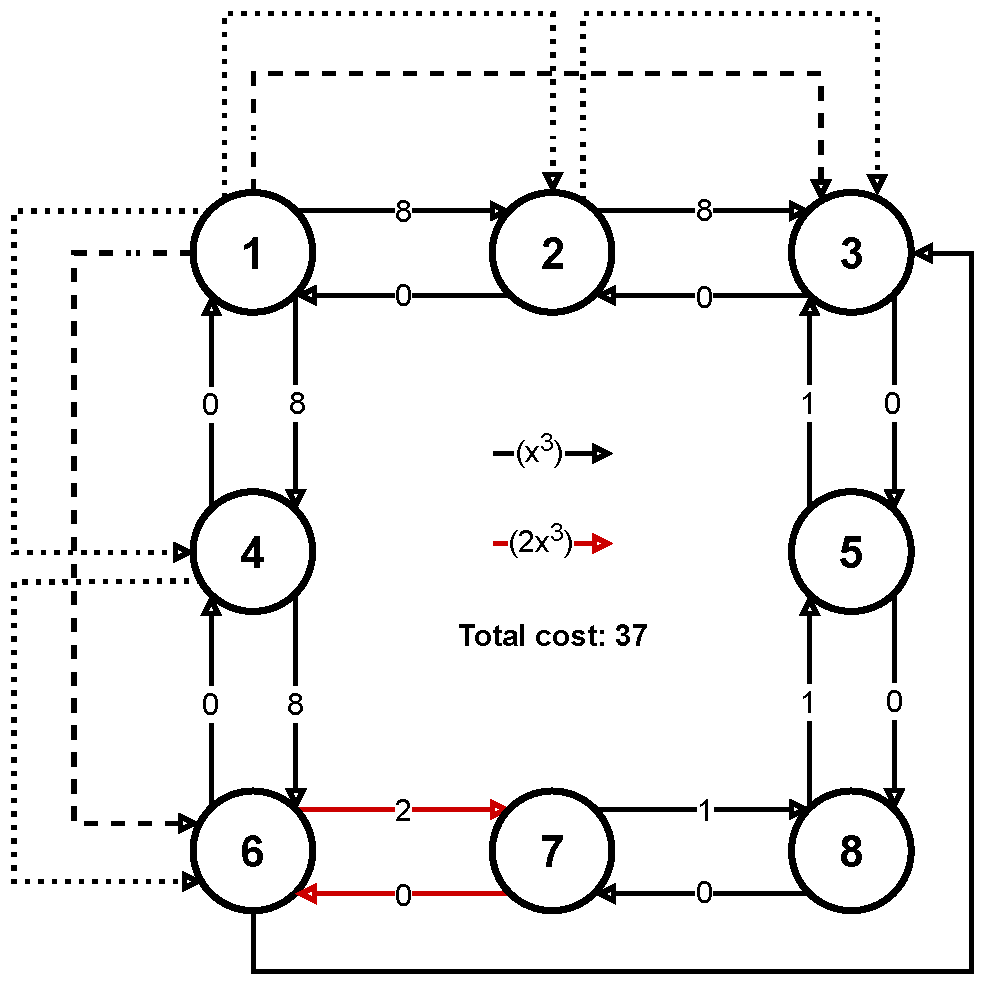
\includegraphics[width=\linewidth]{Img/cex_opt.pdf}
    \end{minipage}
    \captionof{figure}{Instance $4$, its MWU solution, and its optimal solution}
    \label{fig:cex}
}

\begin{figure}[h!]
    \centering
    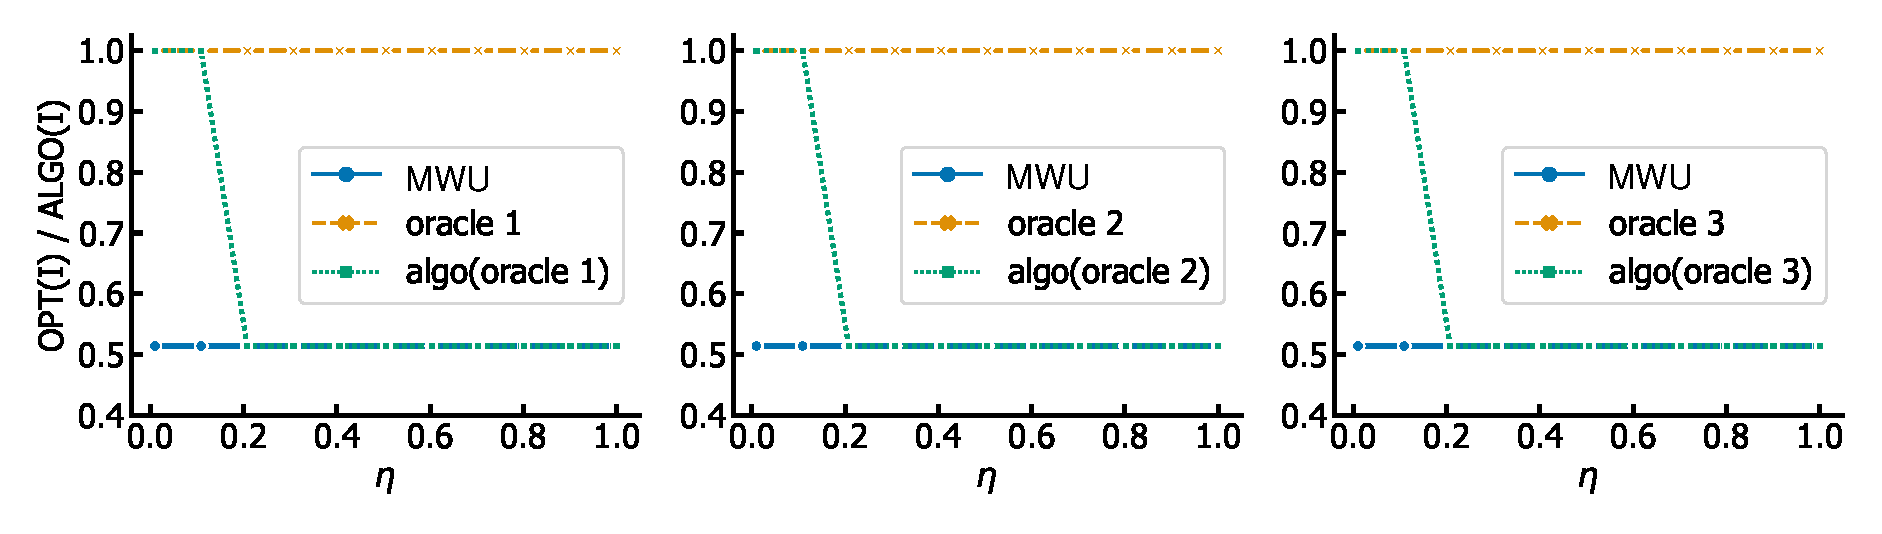
\includegraphics[width=\linewidth]{Img/cex_tight.pdf}
    \caption{Performance analysis of Instance $4$}
    \label{fig:cex-perf}
\end{figure}


\begin{figure}[h!]
    \centering
    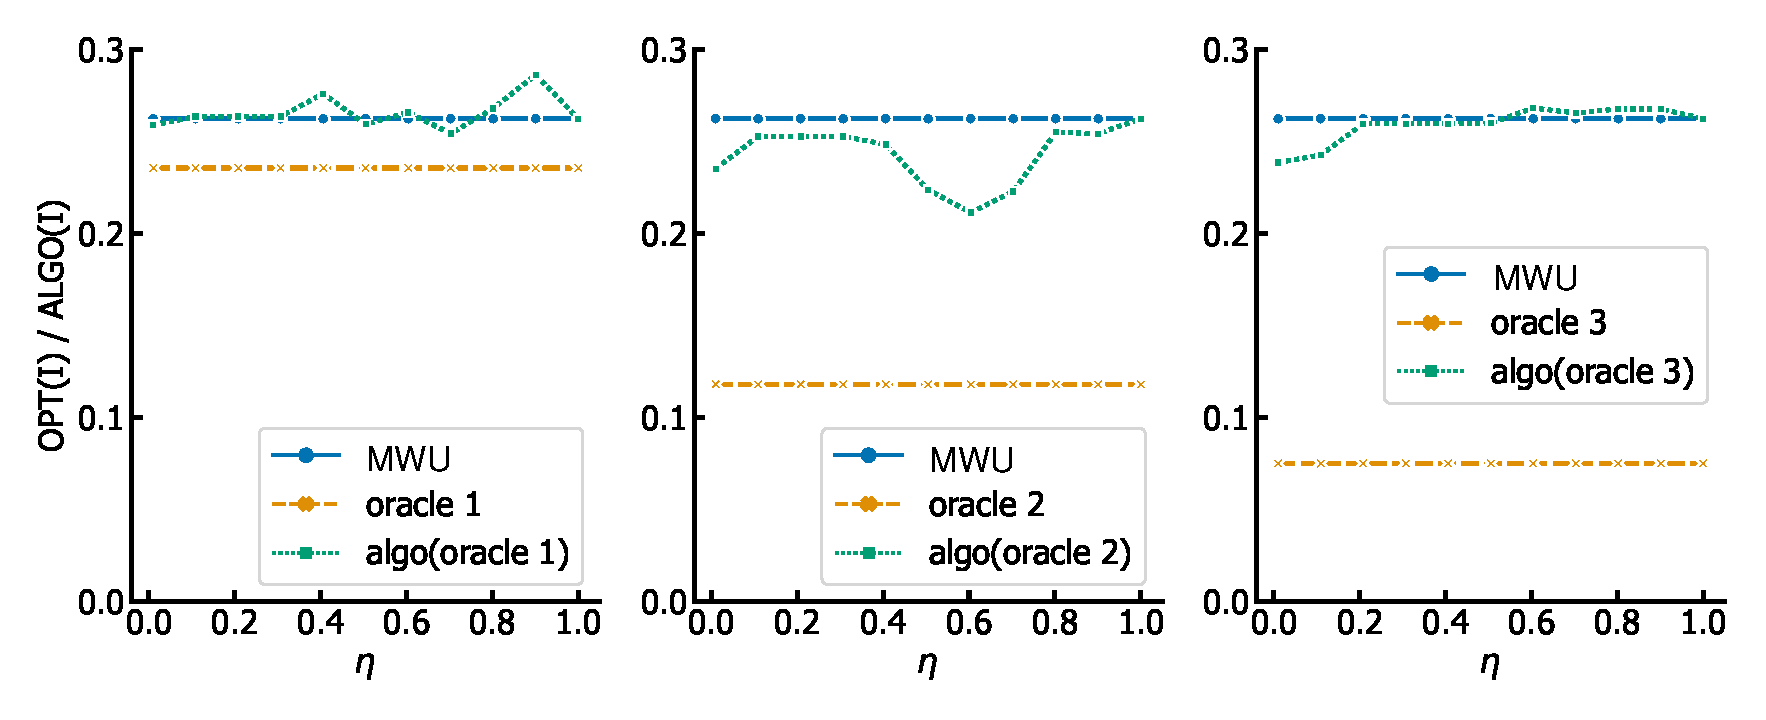
\includegraphics[width=\linewidth]{Img/random_tight.pdf}
    \caption{Performance analysis of Instance $1$}
    \label{fig:random}
\end{figure}


\begin{figure}[h!]
    \centering
    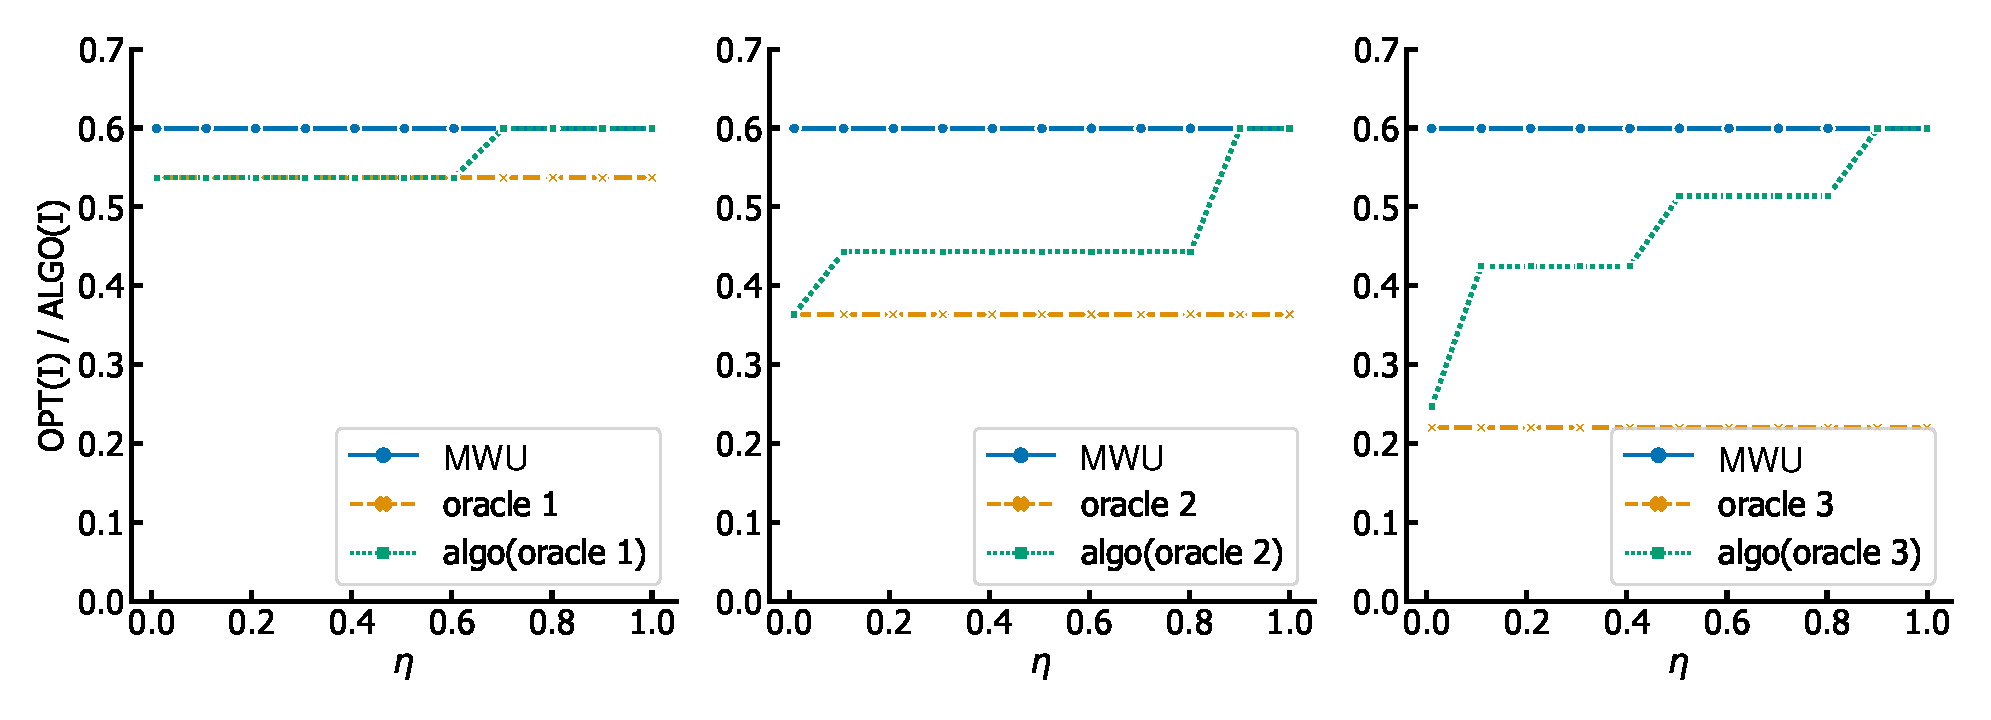
\includegraphics[width=\linewidth]{Img/random_small_tight.pdf}
    \caption{Performance analysis of Instance $2$}
    \label{fig:small-random}
\end{figure}

\begin{figure}[h!]
    \centering
    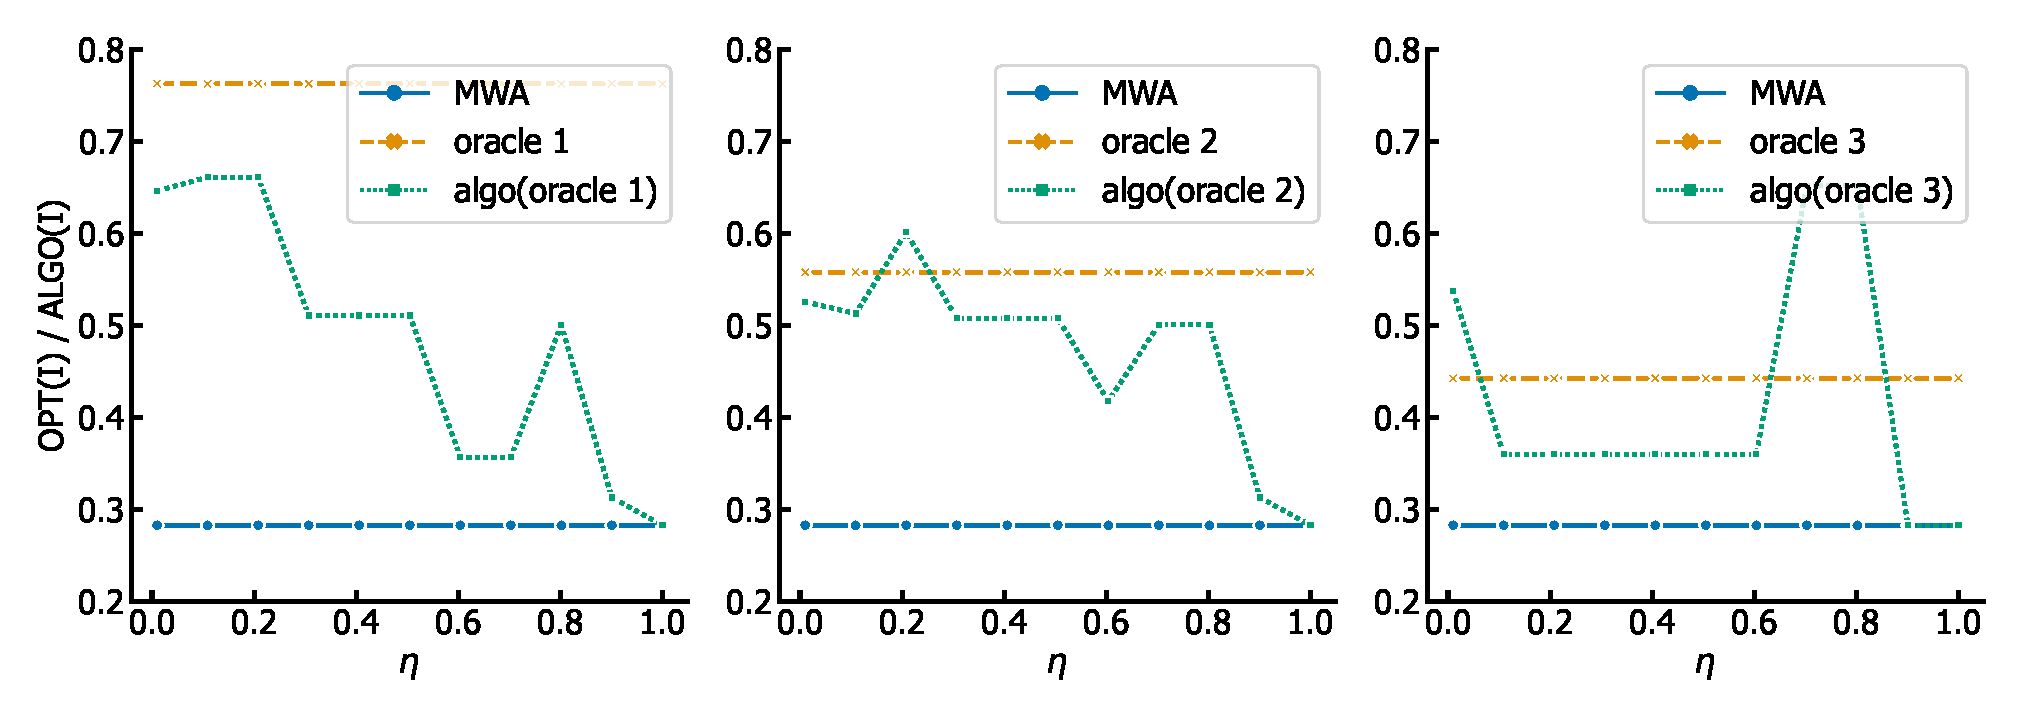
\includegraphics[width=\linewidth]{Img/connected_tight.pdf}
    \caption{Performance analysis of Instance $3$}
    \label{fig:connected}
\end{figure}
